% !TEX root = ../../thesis.tex

\chapter{Exploring the role of morphology with Poppy} % (fold)
\label{cha:exploring_the_role_of_morphology}


Poppy has been designed to be a new experimental platform opening the possibility to systematically study the role of morphology in sensorimotor control, in human-robot interaction and in cognitive development. Indeed, as we discussed in chapter REF, a suitable design of a robot morphology can greatly simplify control problems, increase robustness, and open new modes of interaction with the physical and social world. Thus, being able to study the body as an experimental variable, something which can be systematically changed and experimented, is of paramount importance. Yet, until recently it was complicated because building a robot relied on heavy and costly manufacturing techniques. 3D printing has changed the landscape of what is possible: Poppy Project transposed it to humanoid robotics, and it is now possible to explore new body shapes in just a few days. In addition, its size, weight and power actuation highly reduce the risk of self-damage if a programming error occurs, which means experimentation can be directly conducted in the real world without having to either use physical simulator or build heavy experimental setup.

As an application of the methodology presented in the chapter REF, and especially interested by the role of morphology in the understanding of biped locomotion, we decided to use Poppy to explore the impact of particular leg design on bipedal stability.

In this chapter, we suggest to explore the impact of the thigh shape on the lateral stability(see section~\ref{sec:experimental_thigh_shape}) and evaluate the efficient of foot designs for balance and biped locomotion.

% !TEX root = ../../thesis.tex

\section{Evaluation of the role of a bio-inspired thigh shape} % (fold)
\label{sec:evaluation-thigh}
Humanoid robots need to be able to move robustly and efficiently in human environments, which includes the ability to keep stability when unpredictable physical contact with humans happens.
This raises new important challenges regarding the robustness and safety of robots in an always changing, unpredictable, and open-ended environment.

While state-of-art humanoid and bipedal walking robots (e.g.Honda Asimo~\cite{hirai1998development} or Kawada Industries HRP robots~\cite{kaneko2008humanoid}) have shown interesting results on the achievement of efficient walking behaviors in a rather specified environment, they did not really explore robustness capabilities in unspecified environment and reactivity under unpredicted events.
Yet, one will have to tackle these challenges to be safely used at home with non-expert users.
Also, their walking behaviors require high speed sensorimotor control loop using inverse dynamic and zero moment point~\cite{kajita2003biped} with precise and powerful actuation.
We think that another interesting way to enable robots to adapt their behaviors to unknown environments is to provide them with control algorithms which can be updated with learning algorithms based either on social guidance~\cite{billard2008robot}, or on autonomous self-exploration~\cite{Baranes2012RAS}.
A part of the computation needed for such adaptation could also be done through the intrinsic mechanics and electronics of the robot, thus providing effective and hyper-responsive reactions while simplifying the algorithms of the different behaviors.
This role of morphology has been called morphological computation~\cite{pfeifer2005morphological}, as the body of the robot becomes a form of information processing structure~\cite{Pfeifer06}, able to support a part of the computation necessary to achieve sensorimotor tasks to simplify or make it more robust to external disturbances~\cite{Pfeifer07}.
The actions or reactions of the physical body also have the advantage of being direct without latency due to a controller, as opposed to CPU computed reactions which often require high-cost hardware in order to respond fast enough and reduce modeling errors.


\begin{figure}[!t]
\centering
    \subfloat[][bended thighs]{\label{fig:poppy_with_bended_legs}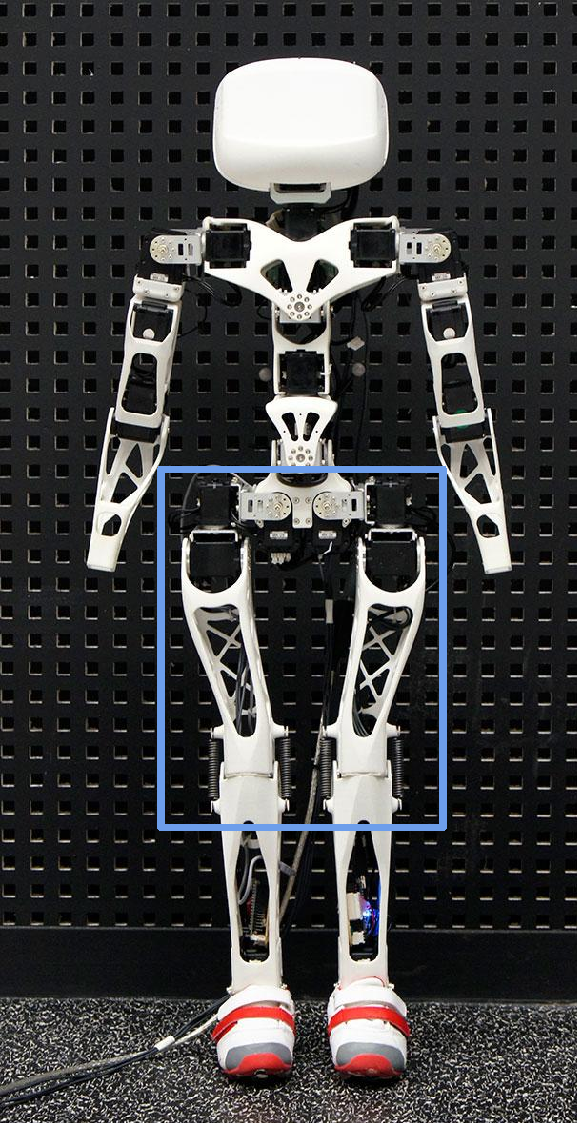
\includegraphics[width=0.42\linewidth]{poppy_bended_tigh_square.pdf}}
    \hfil
    \subfloat[][straight thighs]{\label{fig:poppy_with_classical_legs}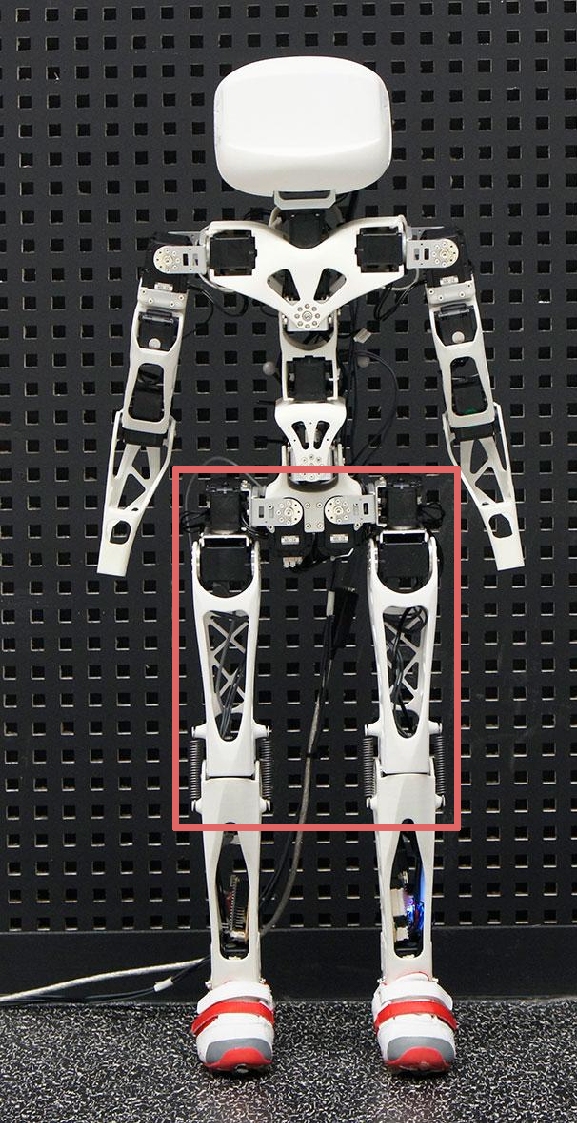
\includegraphics[width=0.42\linewidth]{poppy_straight_tigh_square.pdf}}
    \caption{We evaluate the effect of the thigh morphology on the biped locomotion dynamic.
    Experiments are made using the Poppy humanoid platform.
    In this paper, we compare two thigh morphologies: (a) thigh bended by an angle of 6\textsuperscript{o} and (b) a more classical approach with straight thighs.}
    \label{fig:poppy_compared}
\end{figure}

Within this context we built a whole new humanoid robot called Poppy (see Fig.~\ref{fig:poppy_with_bended_legs}) presented with details in~\cite{lapeyre2013poppy}.
This humanoid robot was designed to easily and quickly conduct scientific experiments on sensorimotor learning, exploring morphology properties, and human-robot interaction.
As an experimentation robotic platform, Poppy was designed to be \textbf{affordable}, \textbf{lightweight}, \textbf{robust and safe}, \textbf{easy to use}, \textbf{versatile} and \textbf{fast and easy to duplicate or modify} with the mid-term goal to make it easily reproducible by other lab through an OpenSource distribution (hardware and software).
This was achieved thanks to 3D printing techniques, affordable off-the-shell components and optimized mounting design.

Its morphology is optimized on the locomotive system (legs and trunks) to increase the robot robustness, agility and stability during the walking.
This is ensured by a combination of an anthropomorphic morphology, morphological computation, articulated spine and lightweight/soft material.
Poppy's morphological properties are theoretically described in~\cite{lapeyre2013poppy}.
In this paper we will focus on its bio-inspired thigh shape, bended by an angle of 6\textsuperscript{o}.
We will investigate the impact of this thigh design on the balance and biped locomotion using a comparison with a more traditional straight thigh (see Fig.~\ref{fig:poppy_compared}).

In the rest of the paper, we will first review current studies on the role of the morphology for biped locomotion.
Then we will present an overview of morphological properties and detail the design of the thigh morphology.
Afterwards we will present experiments we did to compare the current thigh shape (see Fig.~\ref{fig:poppy_with_bended_legs}) with a more classical approach to humanoid leg morphology (see Fig.~\ref{fig:poppy_with_classical_legs}) and finally present and discuss results showing the impacts of its morphology on biped locomotion dynamic.

\subsection{Effect of the bended thigh} % (fold)
\label{sub:effect_of_the_bended_thigh}
If we look closely at the human morphology of the femur, it appears that it is inclined of
6\textsuperscript{o}.
This makes the feet closer to the projection of the center of gravity (see
Fig.~\ref{fig:human_thigh}).
This approach leads to two main stability enhancements during the
walking gait:

\begin{figure}
\centering
    \subfloat[][]{\label{fig:human_thigh}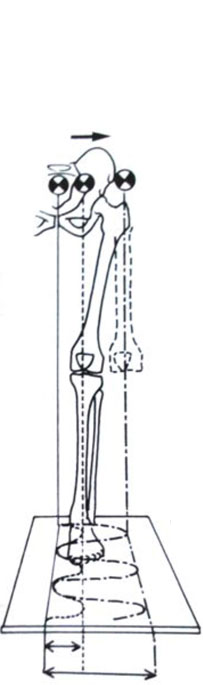
\includegraphics[height=6.5cm]{human_thigh.jpg}}
    \hfil
    \subfloat[][]{\label{fig:model_thigh}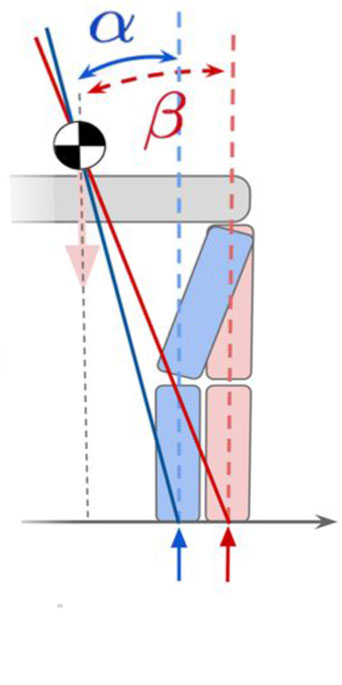
\includegraphics[height=6.5cm]{model_thigh.jpg}}
    \hfil
    \subfloat[][]{\label{fig:thigh_of_poppy}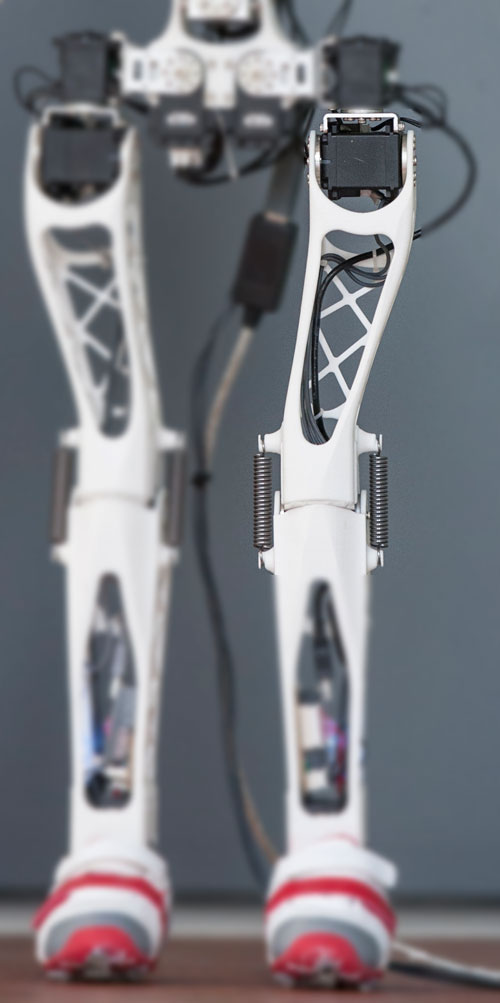
\includegraphics[height=5cm]{thigh_shape_large.jpg}}
    \caption{ a) Effect of the human being bended femur on the human biped locomotion.
    b) Model used for the comparison of the two thighs morphology.
    c) Actual realization of the bended thigh on the poppy platform}
    \label{fig:poppy_thigh}
\end{figure}

\subsubsection{Reduce the falling speed during single support phase} % (fold)
\label{ssub:recude_the_lateral_falling_speed}

We can model the situation where the robot is on one foot by an inverted pendulum with a point mass centered on the center of gravity (CoG) of the robot and the axis of rotation located at the foot position (see Fig.~\ref{fig:thigh_of_poppy}).
The dynamic of the whole structure depends on:

\begin{itemize}
    \item the length $l$ of the segment extending from the foot to the center of gravity,
    \item the angle $\theta$ of the segment relative to the vertical,
    \item the gravity force $g$.
\end{itemize}

The system follows the law:

$$\ddot{\theta}(t) + w_0 \cdot sin(\theta(t)) = 0$$
$$w_0 = \sqrt{\frac{g}{l}}$$

To get a first idea of the behavior, we can linearize the system for small disturbance such as:

$$\theta(t) = \theta_0 \cdot cos(w_0\cdot t)$$
$$\dot{\theta}(t) = -\theta_0 \cdot w_0 \cdot sin(w_0\cdot t)$$

The position and velocity of the pendulum linearly varies with the initial $\theta$ angle.
Reducing
this initial angle $\theta_0$ involves a direct reduction of the falling speed $\dot{\theta}(t)$ of
the robot.

In the case of Poppy's geometry, the thigh bending allows a 40\% reduction of the initial
angle $\theta_0$ ($\alpha = 3.8$\textsuperscript{o} against $ \beta = 6.4$\textsuperscript{o} on
Fig.~\ref{fig:model_thigh}).

In the case of a fall, it is not possible to respect the assumption of small perturbations, that is
why we have simulated the model in Matlab with a non-linear system.
We obtain the behavior
represented in Fig.~\ref{fig:dynamic_thigh_model}.

\begin{figure}[thpb]
    \centering
    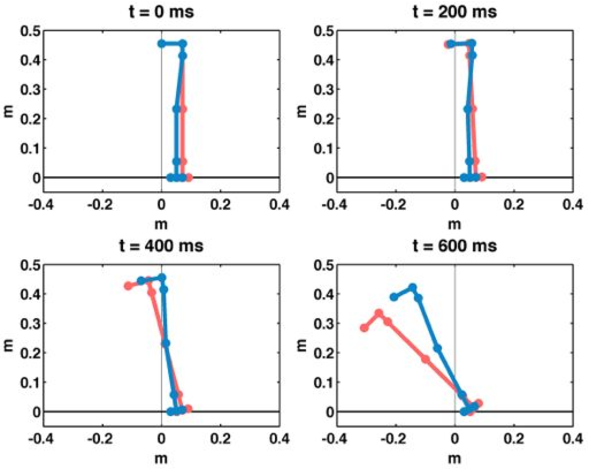
\includegraphics[width=6cm]{dynamic_thigh_model.pdf}
    \caption{Comparison of the falling dynamic over time when Poppy is standing on one foot depending on  its thigh morphology: with a bended thigh of 6\textsuperscript{o} (blue) and with a straight thigh (red).}
    \label{fig:dynamic_thigh_model}
\end{figure}

If we define the center of gravity altitude as:
$$ z_{CoG} = l \cdot cos(\theta(t)) $$


We can express its falling speed over time as:

$$ \dot{z}_{CoG} = - \dot{\theta}(t) \cdot l \cdot sin(\theta(t))$$


The simulation shows that between 0 and 700ms, the mean of the CoG falling speed is reduced by 56\%.
% subsubsection recude_the_lateral_falling_speed (end)

\subsubsection{Reduce the lateral translation of the center of gravity during double stance phase} % (fold)
\label{ssub:reduce_the_lateral_translation_of_the_center_of_gravity}

As the feet are closer to the gravity center, the necessary lateral translation of the CoG to transfer the mass of the robot from one foot to another is reduced (see Fig~\ref{fig:human_thigh}).
In the case of Poppy's morphology, thanks to the $6$\textsuperscript{o} bended thigh, the lateral motion of the CoG is reduced by about 30\% ($ 5 cm$ instead of $7.1 cm$).

% subsection effect_of_the_bended_thigh (end)

\subsection{Experiments} % (fold)
\label{sub:experiments}
The simple model described in the previous section showed that a slight inclination
(6\textsuperscript{o}) of the thigh can theoretically have a significant gain regarding the lateral
stability of the robot during the two main phases of the walking gait (i.e.
single stance
phase~\ref{ssub:recude_the_lateral_falling_speed} and double stance
phase~\ref{ssub:reduce_the_lateral_translation_of_the_center_of_gravity}).

In this section, we describe representative experiments which evaluate the actual gain of the thigh
shape on the real Poppy platform.
To do this, we used both a pair of straight thighs and the bended
thighs presented above.
We will compare Poppy's reactions with those different legs (see
Fig.~\ref{fig:poppy_compared}) on three experiments:
\begin{itemize}
    \item Evaluate the falling speed during single support stance.
    \item Measure the lateral translation to move the CoG Form one feet to the other.
    \item Record the upper body motion during biped locomotion.
\end{itemize}

\subsection{Single support falling velocity} % (fold)
\label{sub:falling_velocity}
The experiment evaluates the fall velocity of Poppy when it is supported on only one foot and compare it with the theoretical results obtained in~\ref{ssub:recude_the_lateral_falling_speed}.
To do so, the robot's head is tracked by an Optitrack\footnote{\url{http://www.naturalpoint.com/optitrack/products/v120-trio/}} device and markers are placed on the head.
In postural balance on two feet, a motor order triggers the raise of a foot which unbalances the robot (see Fig.~\ref{fig:falling_experiment_dispositif}) and causes its lateral fall (see Fig.~\ref{fig:fall_of_poppy}).
This experiment was repeated about fifteen times for the two cases studied, i.e.
with bended legs (Fig.~\ref{fig:poppy_with_bended_legs}) and with straight legs (Fig.~\ref{fig:poppy_with_classical_legs}).

\begin{figure}[h]
\centering
    \subfloat[][]{\label{fig:falling_experiment_dispositif}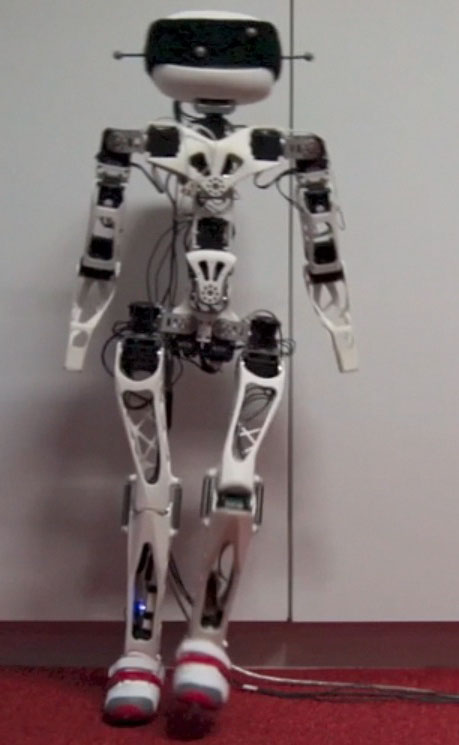
\includegraphics[height=4.2cm]{experience_fall_illu.jpg}}
    \hfil
    \subfloat[][]{\label{fig:fall_of_poppy}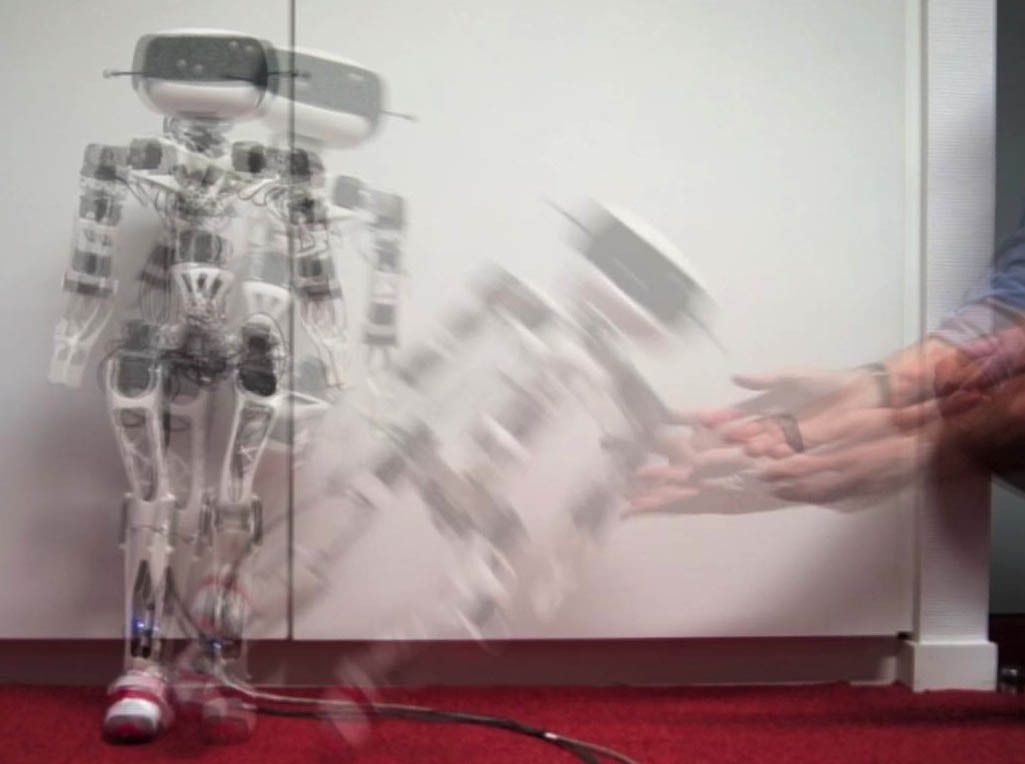
\includegraphics[height=4.2cm]{experience_fall_mean.jpg}}
    \caption{Proceedings of the one support stance falling experiment.
    The Poppy head has a headband with markers to track its absolute position over time.
     a) Initial perturbation done a sudden raise of one foot, b) view of the Poppy lateral fall over time.}
    \label{fig:falling_experiment}
\end{figure}

Experiments results are shown on the Fig.~\ref{fig:falling_results}.
The blue color is assigned to experiments with bended thighs while the red color is assigned to straight thighs.
For each case, the light color corresponds to the standard deviation and the dark color to the 95\% confidence interval of the mean value.
The first figure~(\ref{fig:fall_result_position}) refers to the head altitude position over time
and the second~(\ref{fig:fall_result_velocity}) to the falling velocity of the head.
Dashed lines represent theoretical results obtained with the model presented in section~\ref{fig:model_thigh}.
One can notice the strong similarity both on the shape and on the difference between the two morphologies studied.
Yet, there is a slight time shift between theoretical and experimental results.
This can be explained by the inertia of the real robot which was not take into account during the simulation.

\begin{figure}[h]
\centering
    \subfloat[][Vertical head position]{\label{fig:fall_result_position}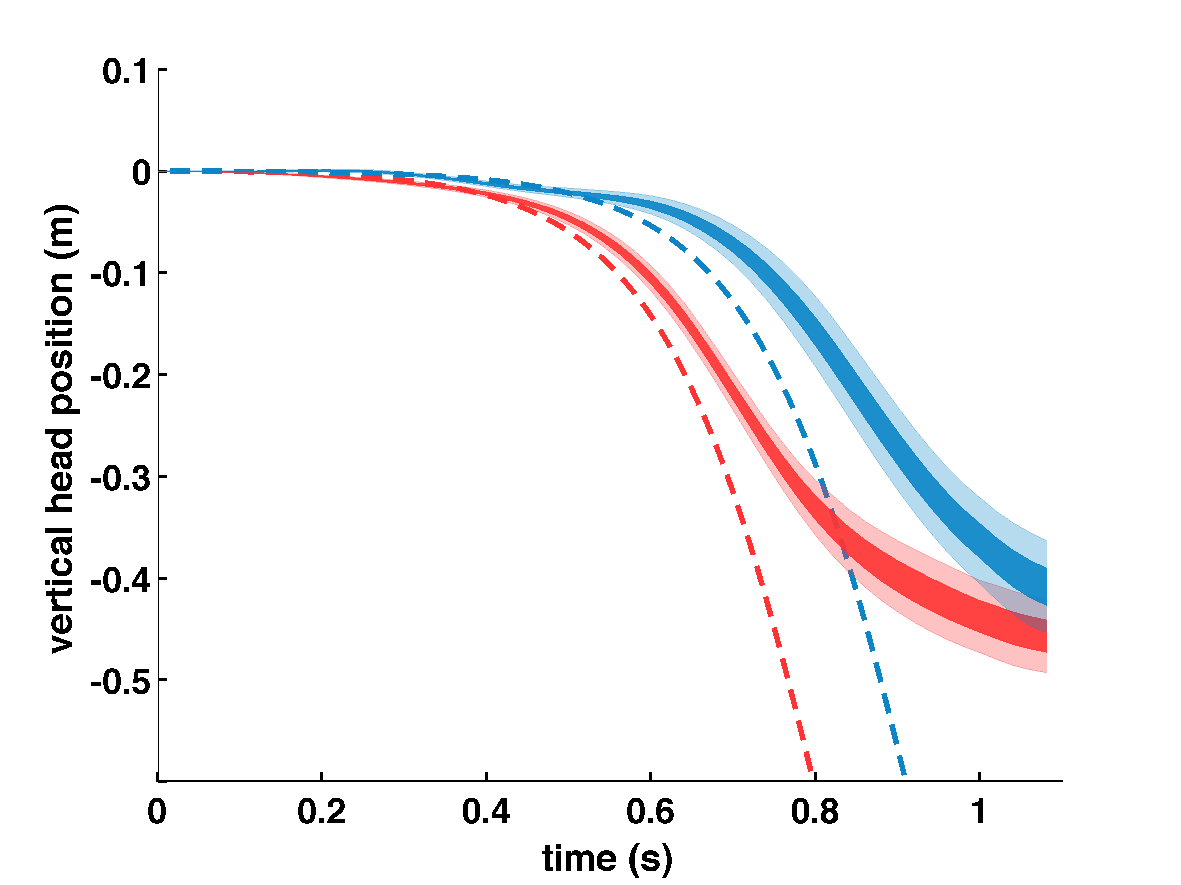
\includegraphics[width=0.49\linewidth]{falling_compare.pdf}}
    \hfil
    \subfloat[][Vertical head falling velocity]{\label{fig:fall_result_velocity}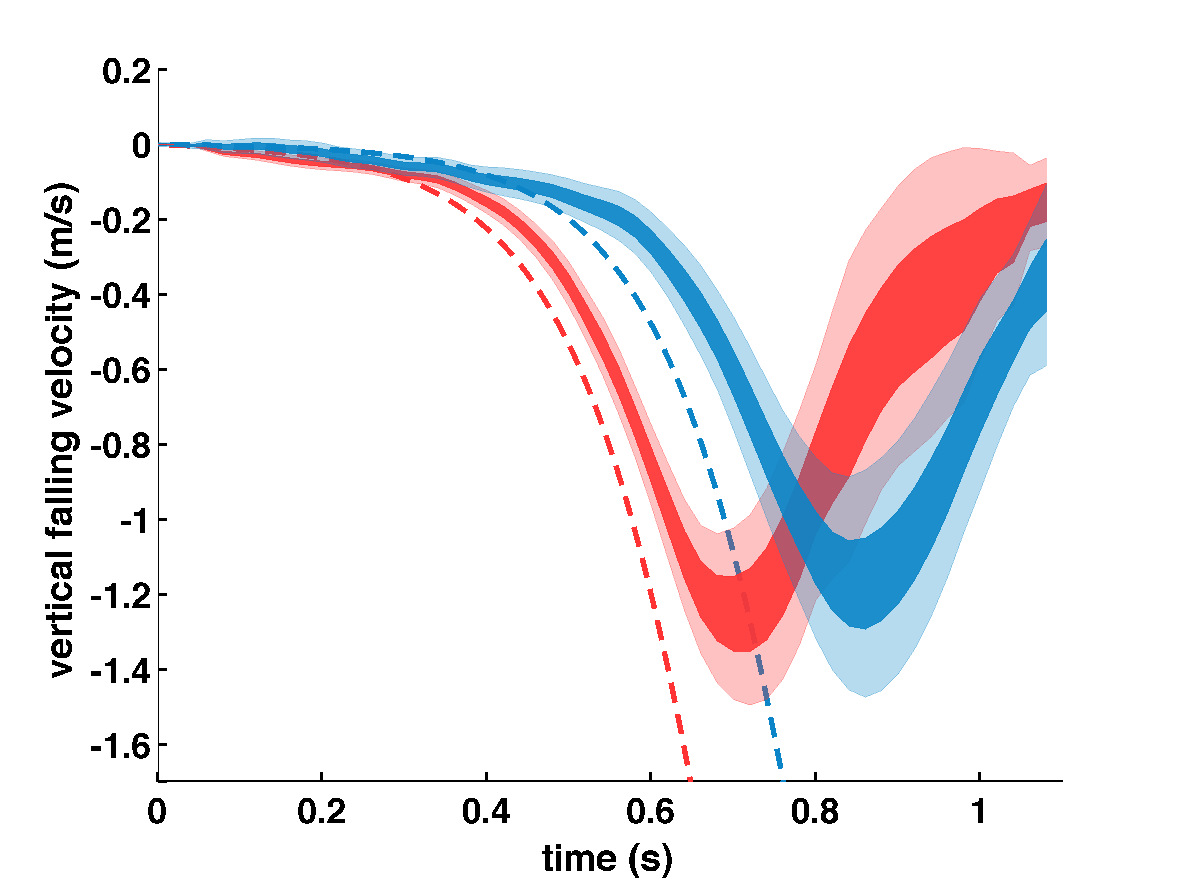
\includegraphics[width=0.49\linewidth]{velocity_compare.pdf}}
    \caption{Results of the single support falling experiment.
    The blue color is associated with experiments conducted with bended thighs while the red color is assigned to straight thighs.
    For each case, the light color corresponds to the standard deviation and the dark color to the 95\% confidence interval of the mean value while dashed lines represent theoretical results.
    These figures shows the vertical position (a) and vertical falling velocity (b) of the head of Poppy over time for each case studied.
    The curves behavior change after 800ms is due to the fact that we catch up the robot before it touches the ground.}
    \label{fig:falling_results}
\end{figure}

These figures show a clear improvement for the Poppy version with bended thigh (blue curves) with a 200ms time shift compared to the straight thigh (as illustrated on the attached video\footnote{\url{http://flowers.inria.fr/Humanoid2013/}\label{video}}).
Thanks to this delay, the falling speed is reduced by about 56\% during the first 700ms.
Thus the robot remains almost stationary for 600 ms (400ms in the case of straight thigh).
The typical walking gait of Poppy is done over a period of one second so the mono-pedal stance phase last around 420 ms~\cite{lapeyre2013poppy}.
Considering that the robot remains stationary during more time than the single stance phase, we can imagine that the lateral balance control will be reduced during the walking gait.

% subsection falling_velocity (end)


\subsubsection{Double support CoG transfer} % (fold)
\label{sub:cog_motion}


In this experiment we evaluate the necessary lateral movement of the robot to cause a displacement
of its center of gravity from one foot to the other and verify the theoretical results obtained
in~\ref{ssub:reduce_the_lateral_translation_of_the_center_of_gravity}.
For this, Poppy is placed on
a force platform to measure the displacement of its center of pressure.
The absolute movements of
the robot are tracked with an OptiTrack device and markers placed at the head and lower back
(approximately the position of the actual center of gravity).
The robot is kept rigid in a neutral
position and a human physically pushed it from left to right until it reaches its lateral falling limit.
As this operation is not very accurate, the experiment is repeated a hundred times.

\begin{table}[h]
\centering
\begin{tabular}{|l|c|c|c|}
  \hline &      Straight tigh &                     Bended Tigh &                   diff(\%) \\
  \hline CoP & 74.6 {\scriptsize$\pm$9.0} mm &     49.8 {\scriptsize$\pm$7.7} mm & 33\\
  Head & 100.1{\scriptsize$\pm$14.4} mm&     62.9{\scriptsize$\pm$22.0} mm &  37\\
  Lower Back & 64.1{\scriptsize$\pm$11.5} mm&      43.4{\scriptsize$\pm$15.0} mm &  32 \\
  \hline
\end{tabular}
\caption{Summary of the results obtained during the experiment on the lateral motion needed to transfer the robot mass from one foot to the other.}
\label{tab:CoG_motion}
\end{table}

The table~\ref{tab:CoG_motion} presents for each area considered (i.e.
center of pressure (under feet), lower back and head motion) the amplitude of the lateral motion (in millimeter) needed to translate the CoG of the robot from one foot to the other for the two versions of the Poppy thigh design.
The last columns summarizes the relative difference between the two conceptions (in percent).
One can note that the results show a reduction of lateral movement of around 30\%.
Thanks to the shape of the thigh, the lateral displacement of the upper body required to move the CoG from one foot to the other can be reduced.


The results presented on the two first experiments show improvement for two main aspects needed during biped locomotion: lateral stability and mass transfer.
In the next experiment, we will evaluate if there is a significant performance gain in a complex dynamic phase such as bipedal walking.

% subsubsection cog_motion (end)


\subsubsection{Walking dynamic} % (fold)
\label{sub:walking_dynamic}

As explained in the introduction and description of the platform, Poppy has been especially designed to study bipedal walking and human-robot interaction.

Here the experiment consists in playing an open-loop walking pattern while the robot is guided through the physical interaction with a human.
The users role is to provide both balance and control of mass transfer.
By producing small lateral motion on the upper-body they can help the robot to move its CoG from one foot to another.

\begin{figure}[h]
    \centering
    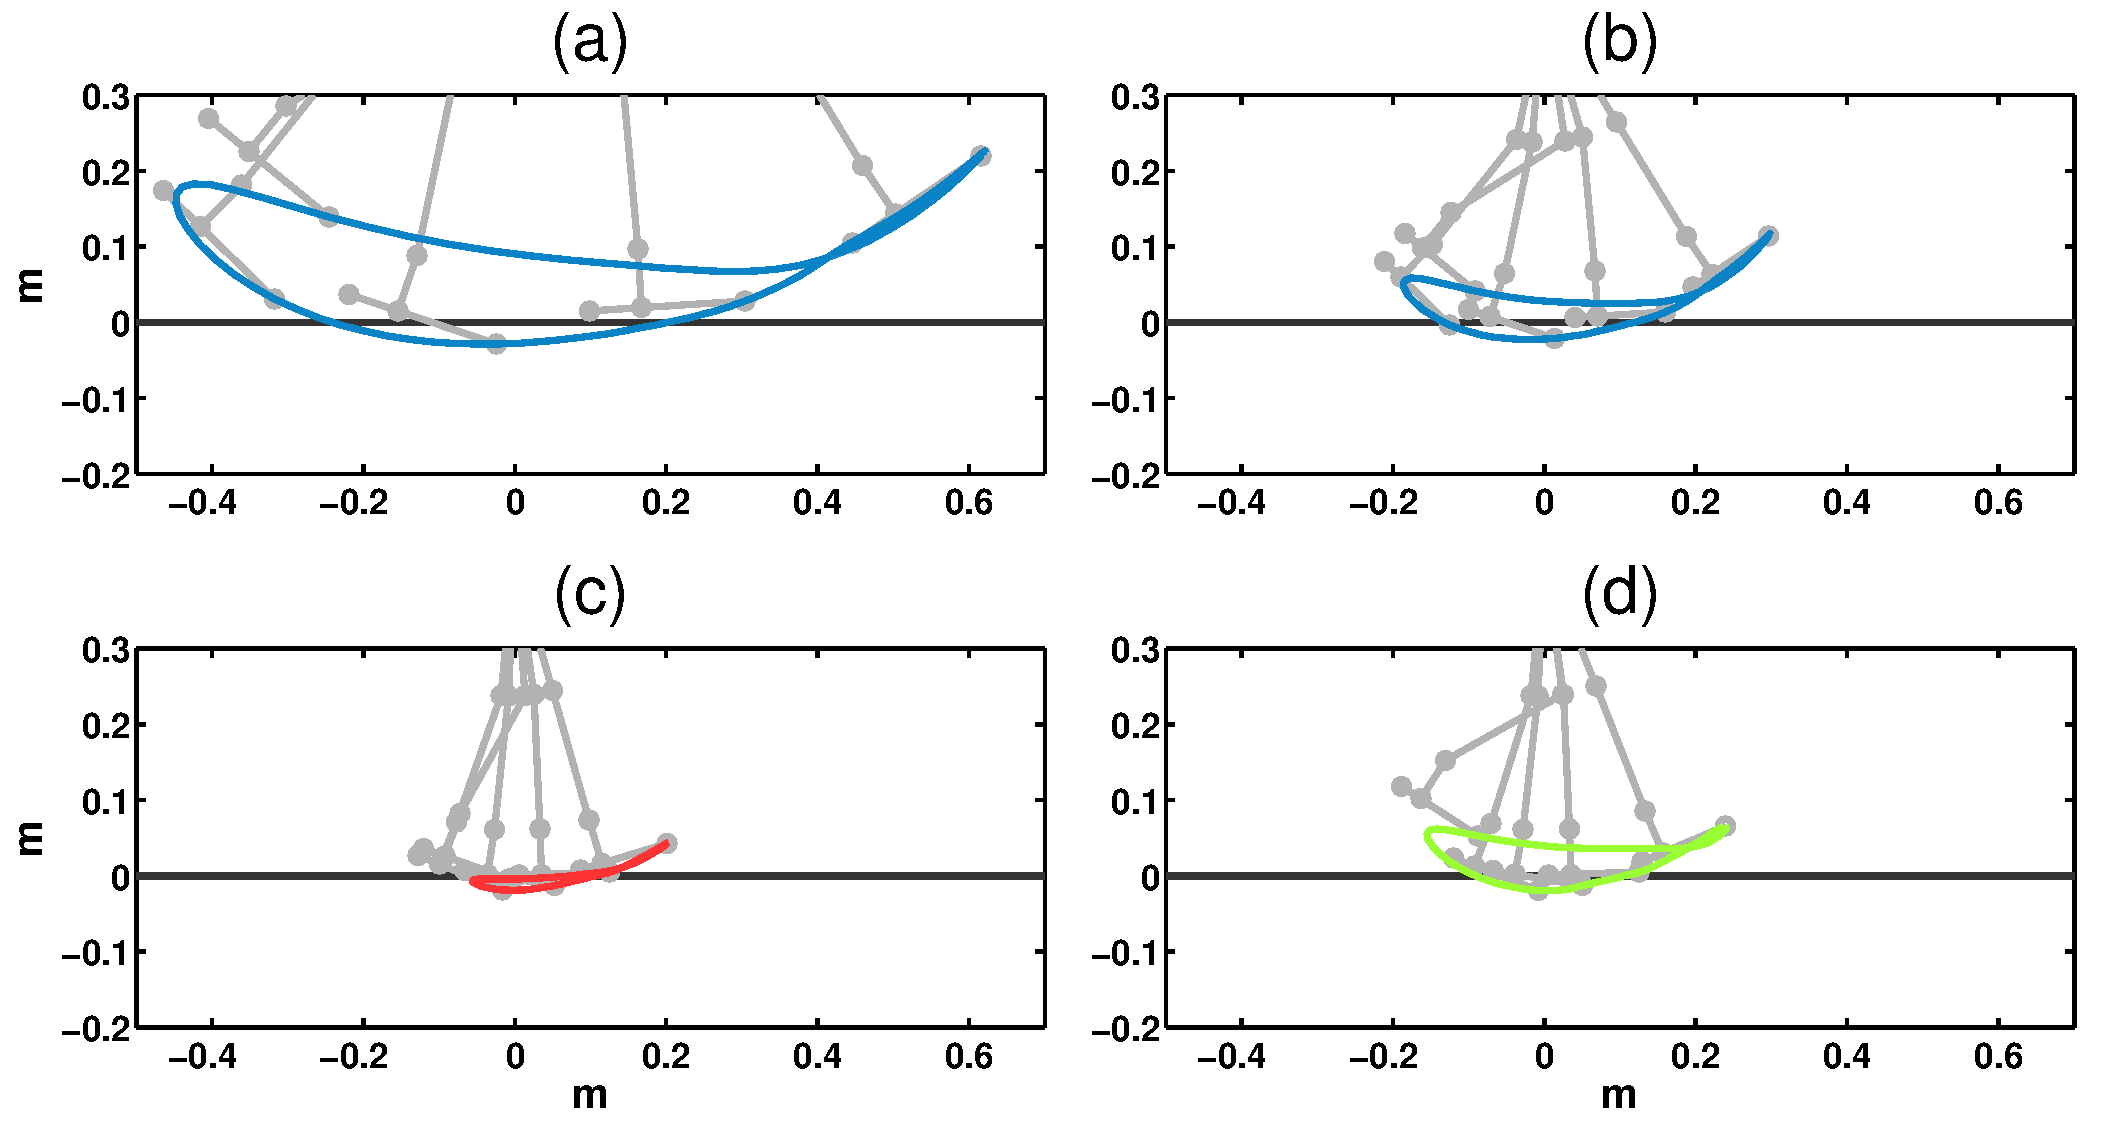
\includegraphics[width=0.95\linewidth]{CPG.pdf}
    \caption{Toes trajectories generated by the walking pattern a) Kinematics of human walking
    with human's morphology b) Direct transposition of the human kinematics with Poppy's morphology
    c) Reducing amplitude of the human kinematics joints with Poppy's morphology d) Walking pattern
    used for the experiment with Poppy}
    \label{fig:CPG}
\end{figure}

The gait is based on the actual human sagittal joint kinematic~\cite{Nester2003}: hip, knee, ankle (see Fig.~\ref{fig:CPG}.a).
A direct transposition of the human joint kinematic on the Poppy's morphology results in a walking speed which is too fast to be handled by users (see Fig.~\ref{fig:CPG}.b).
A simple reduction of joints amplitude conducts to an unsuitable leg trajectory where toes bump into the ground during the swing phase (see Fig.~\ref{fig:CPG}.c).
So to ensure enough clearance during the swing phase and suitable walking speed for the guidance with user, we modified the joints trajectories by hand to both reduce the length step and increase the foot clearance (see Fig.~\ref{fig:CPG}.d).
The actual gait on Poppy is shown on the Fig.~\ref{fig:cpg_on_poppy}.


\begin{figure}[h]
    \centering
    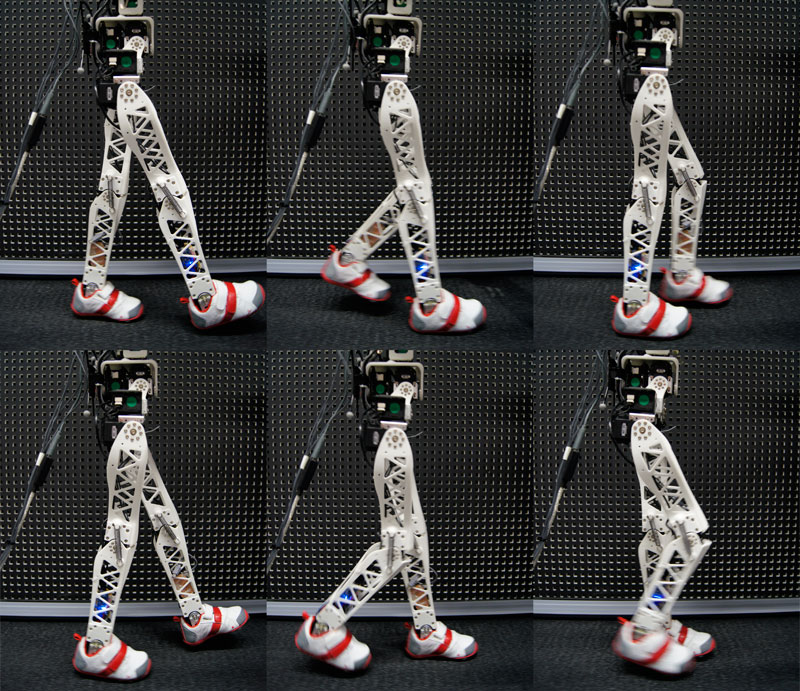
\includegraphics[width=0.7\linewidth]{walking_poppy.jpg}
    \caption{Walking gait CPG described on Fig.~\ref{fig:CPG}.d applied on the actual Poppy robot.
    The CPG generates a human-like walking gait allowing the robot to walk at 1.8km/h and involves straight leg during the stance phase.
    There is no balance control but stability is obtained through physical guidance with trained expert user.}
    \label{fig:cpg_on_poppy}
\end{figure}

In this experiment we are interested by the dynamic of Poppy especially on the frontal plane and we will compare the effect of the thigh shape on this dynamic.
Poppy walks on a treadmill following the walking gait described above.
An expert user trained to keep the robot in the correct walking cycle provides guidance to the robot.
This is done by keeping the robot in a vertical position and supporting, in a compliant manner, the lateral movement of the robot as illustrated in attached videos.
The user is asked to do the best he can to minimize the movement/forces he applies in both morphologies to reduce the bias towards the two design experimented.
All proprioceptive sensors are recorded at 50hz while an Optitrack device associated to markers located at the head and lower back measure the absolute displacements of the robot (voir Fig.~\ref{fig:walking_experiment}).

\begin{figure}[!h]
    \centering
    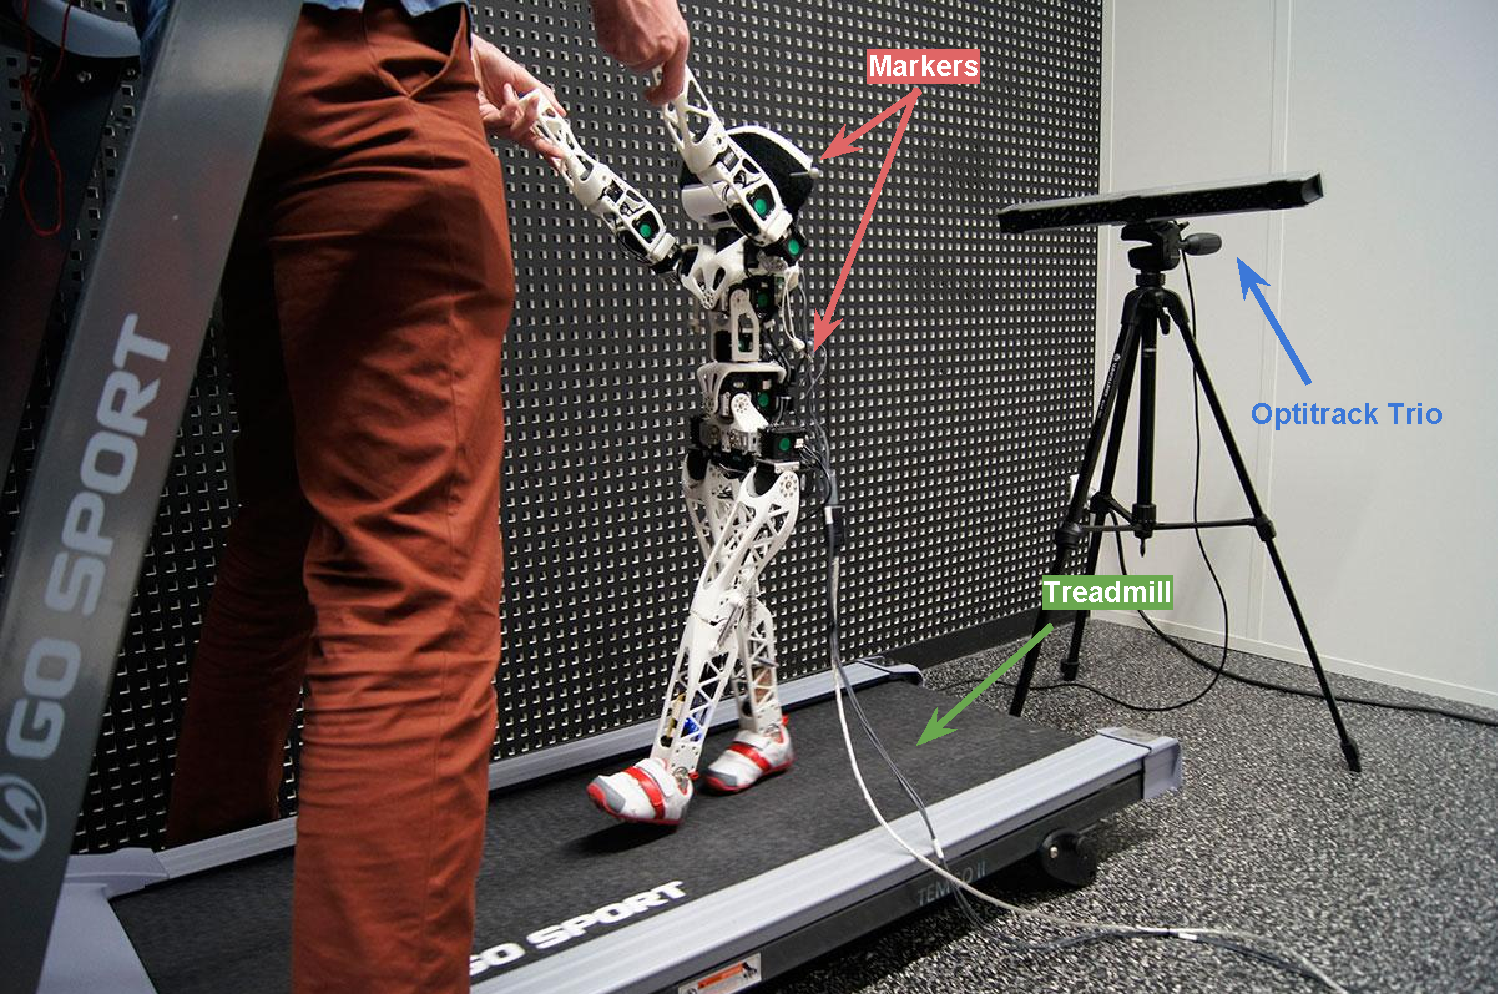
\includegraphics[width=8cm]{dispositif_experience_marche.pdf}
    \caption{Proceeding of the walking experiment.
    Poppy is tracked by an Optitrack trio while it is walking on a treadmill set at 1.8km/h.
    An expert user provides the sagittal balance needed during all the experiment.}
    \label{fig:walking_experiment}
\end{figure}

The Poppy dynamic is recorded for around 1800 walking gait cycle for each thigh design (around 90,000 data points for each case).
Data are folded over to extract the gait behavior over a gait cycle.
Results are presented on Fig.~\ref{fig:walk_result}.
As previously, the blue color is assigned to experiments with bended thigh, the red color is assigned to straight thigh.
For each case, the light color corresponds to the standard deviation and the dark color to the 95\% confidence interval of the mean value.


\begin{figure}[h]
    \subfloat[][Lateral head displacement]{\label{fig:head_position}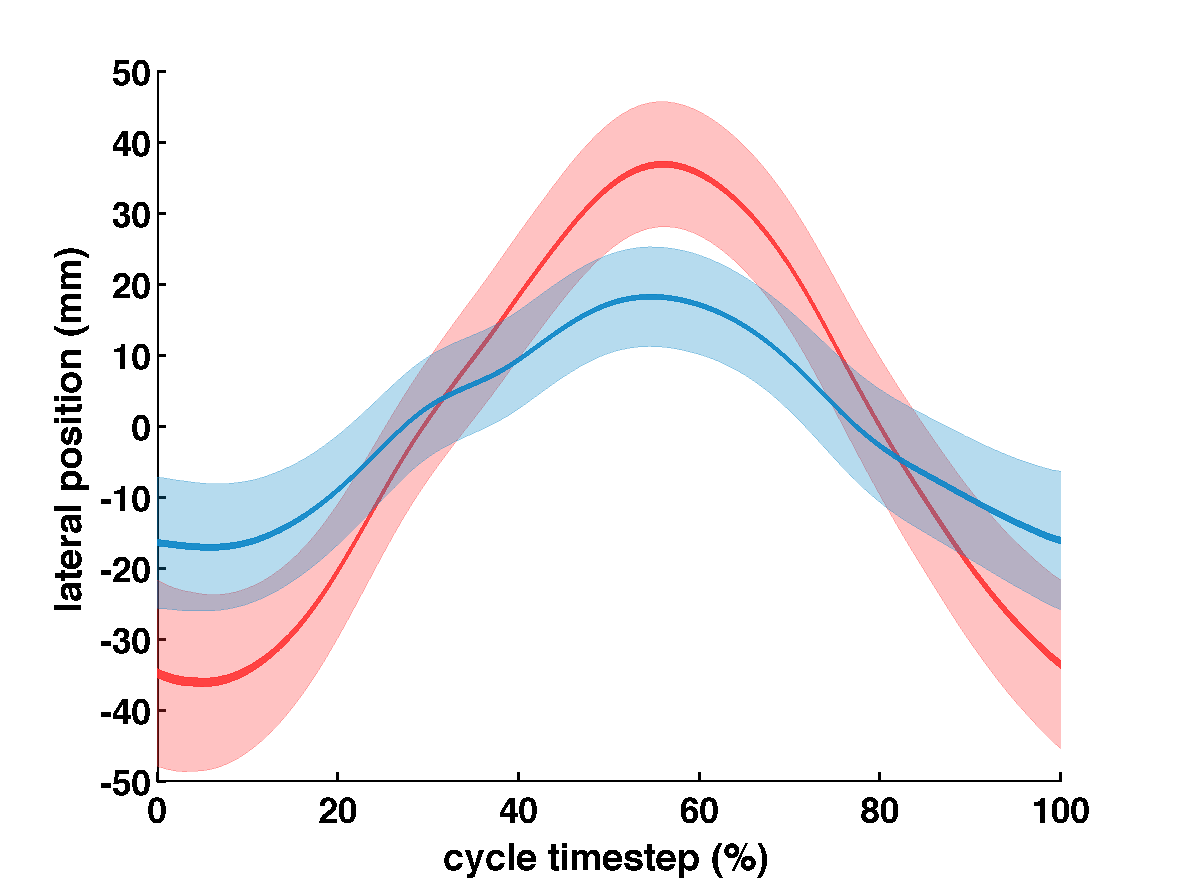
\includegraphics[width=0.49\linewidth]{marche_head_motion.pdf}}
    \hfil
    \subfloat[][Lateral lower back displacement]{\label{fig:low_back_position}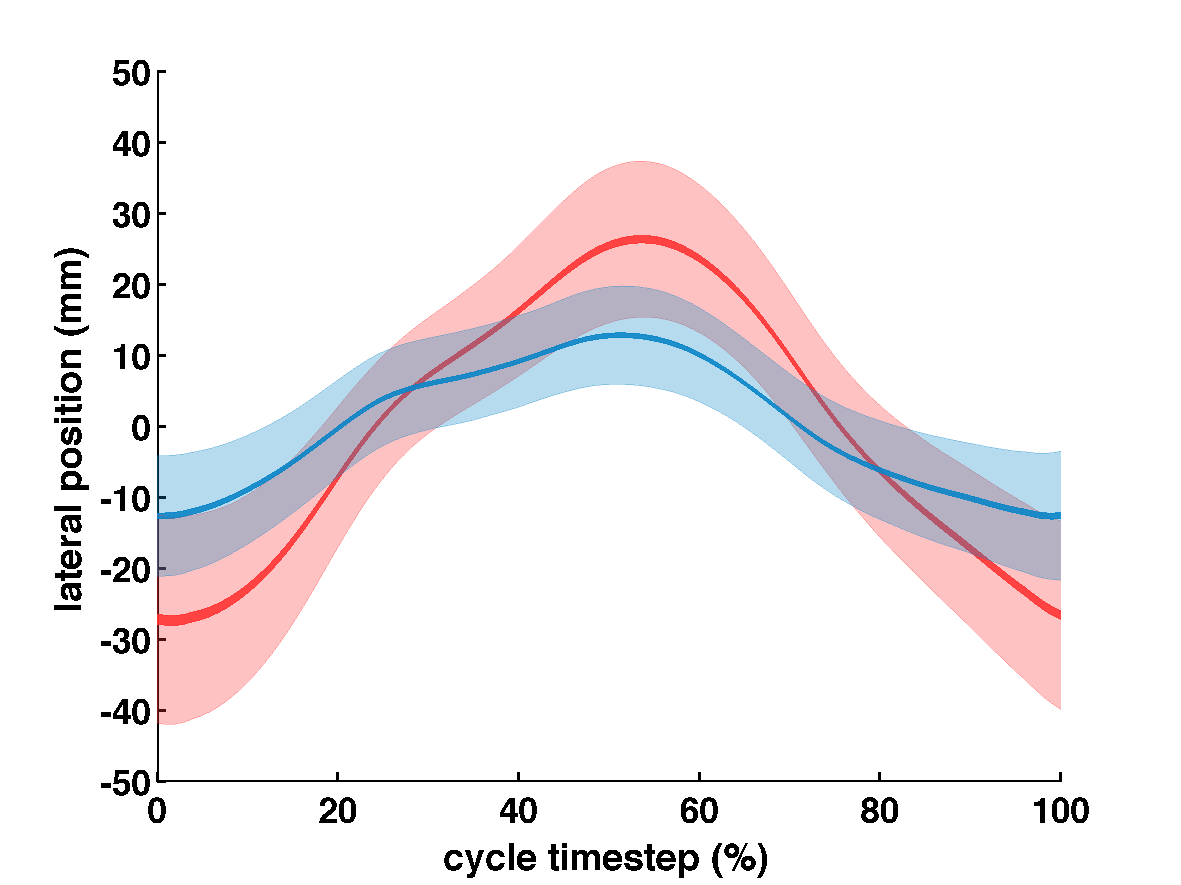
\includegraphics[width=0.49\linewidth]{marche_low_back_motion.pdf}}
    \hfil
    \subfloat[][Sagittal head acceleration]{\label{fig:head_acceleration_x}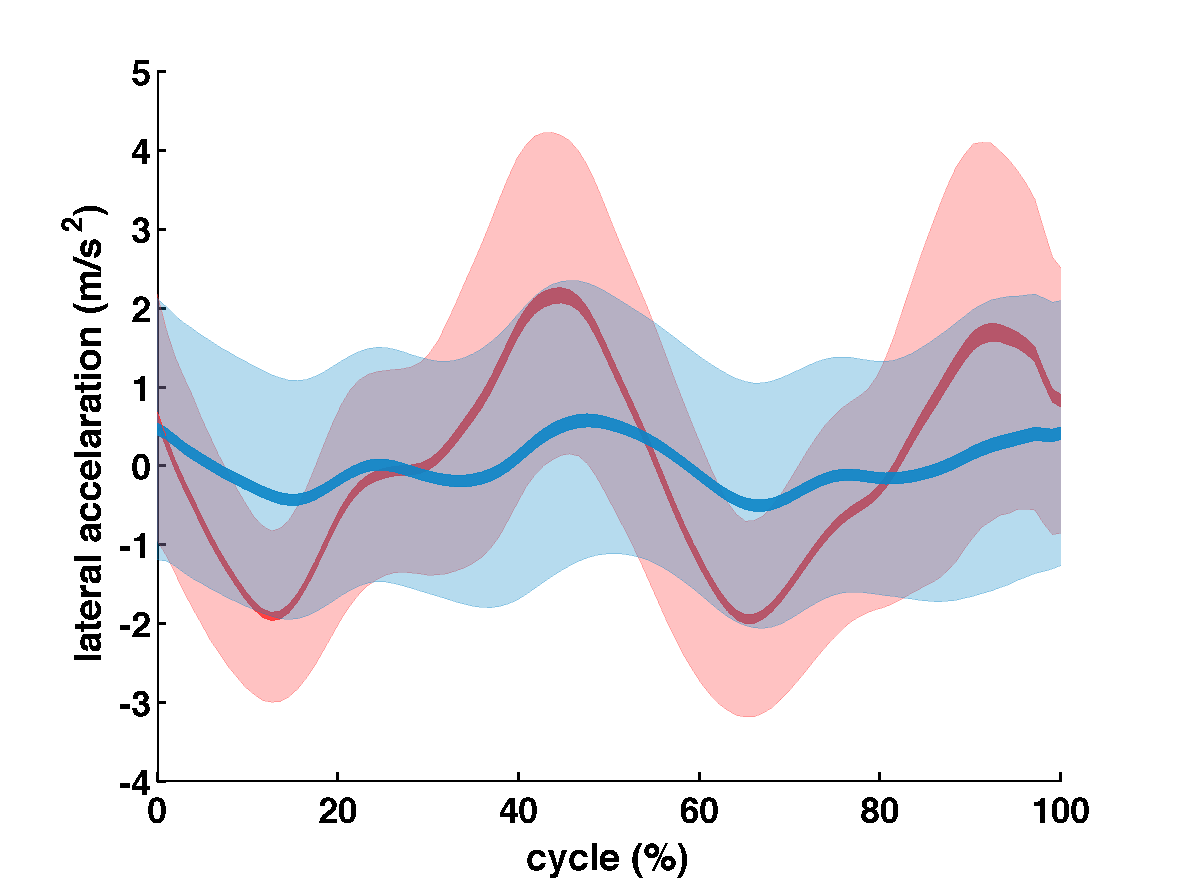
\includegraphics[width=0.49\linewidth]{marche_accel_x_signal.pdf}}
    \hfil
    \subfloat[][Lateral head acceleration]{\label{fig:head_acceleration_y}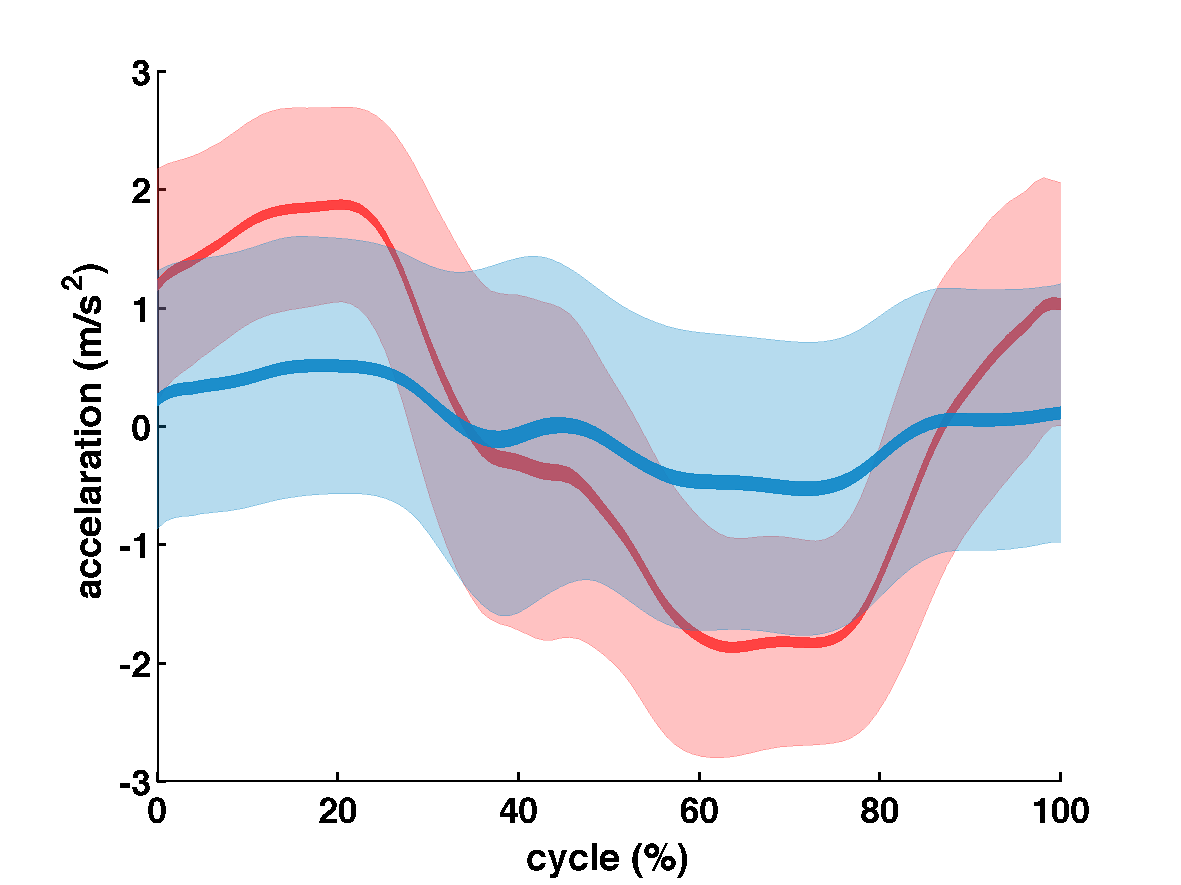
\includegraphics[width=0.49\linewidth]{marche_accel_y_signal.pdf}}
    % \hfil % \subfloat[][Speed of rotation in the frontal plane]{\label{fig:head_gyro_x}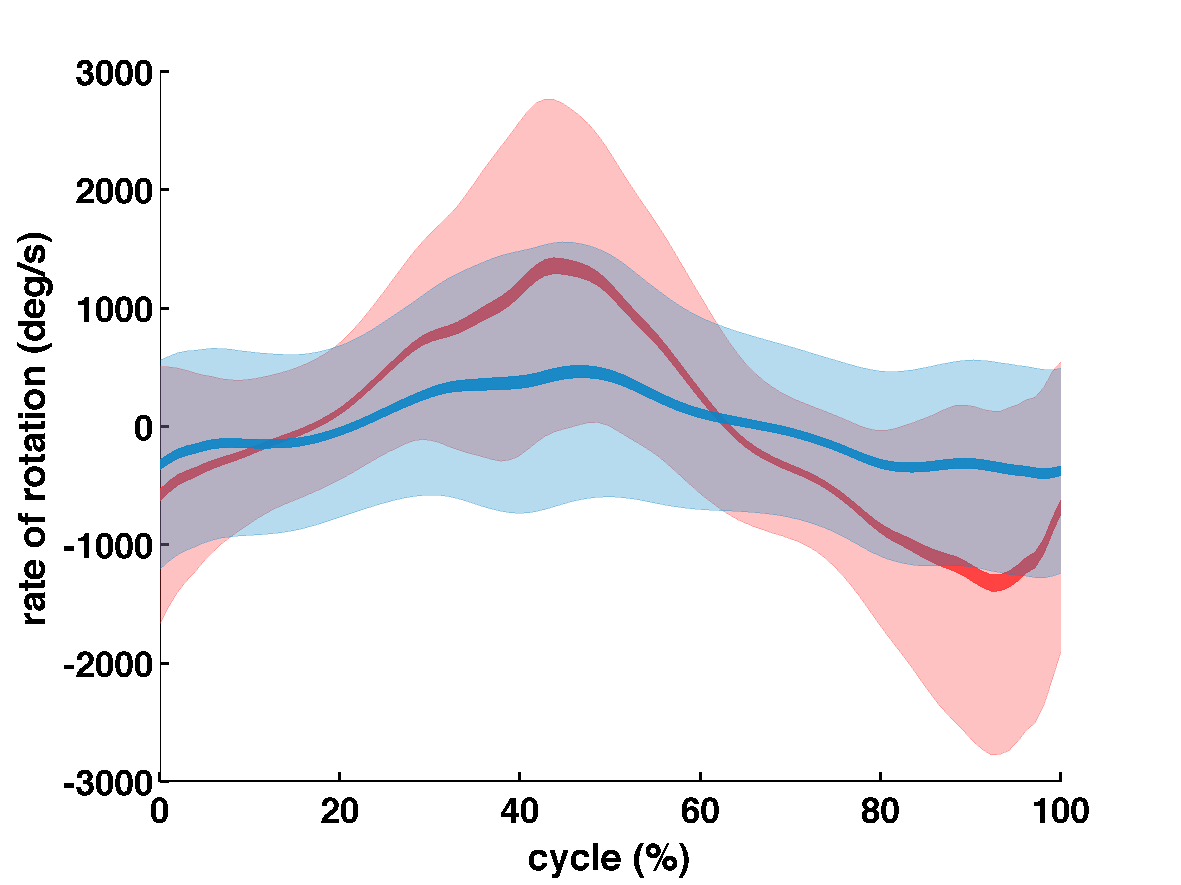
\includegraphics[width=0.32\linewidth]{marche_tilt_x_signal.pdf}}
    % \hfil % \subfloat[][Head inclinaison]{\label{fig:head_tilt_x}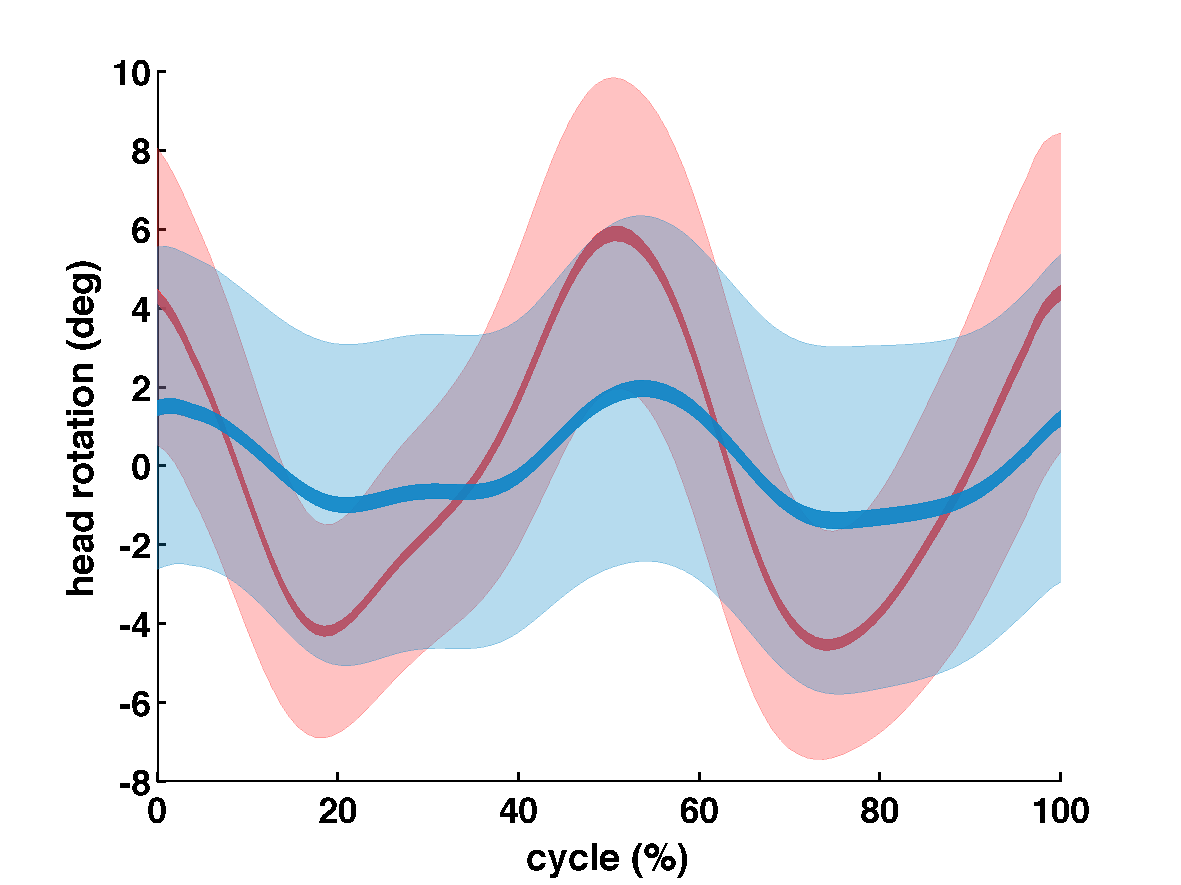
\includegraphics[width=0.32\linew idth]{marche_tilt_y_signal.pdf}}
    \caption{Results obtained during the walking experiment.
    The blue color is associated with experiments conducted with bended thighs while the red color is assigned to straight thighs.
    For each case, the light color corresponds to the standard deviation and the dark color to the 95\% confidence interval of the mean value.
    All data are folded over to extract the mean gait behavior and its standard deviation over a walking gait cycle expressed in percent.}
    \label{fig:walk_result}
\end{figure}

The two first figures (i.e.
~\ref{fig:head_position} and ~\ref{fig:low_back_position}) show the upper body lateral motion in millimeter over the gait cycle.
We can notice that for the two designs, the motion pattern shown by the upper body (head and lower back) is similar.
However in the case of the bended thigh (blue) the amplitude of the motion is reduced by about 45\%.
Another interesting effect concerns the head perturbations shown on figures ~\ref{fig:head_acceleration_x}, and ~\ref{fig:head_acceleration_y}.
Here also, patterns are similar but in the case of the bended thigh the head is clearly less perturbed by the walking dynamic with a reduction in amplitude of approximately 30\%.

Five pictures have been taken while Poppy was walking and were stacked on Fig.~\ref{fig:poppy_walking_compared}.
This shows a qualitative point of view of the walking dynamic for both studied case.
We can notice that the lateral motion of the version of Poppy with bended thigh~\ref{fig:poppy_walking_bended} is small compared to the version with straight thigh~\ref{fig:poppy_walking_straight}.


\begin{figure}
\centering
    \subfloat[][bended thigh]{\label{fig:poppy_walking_bended}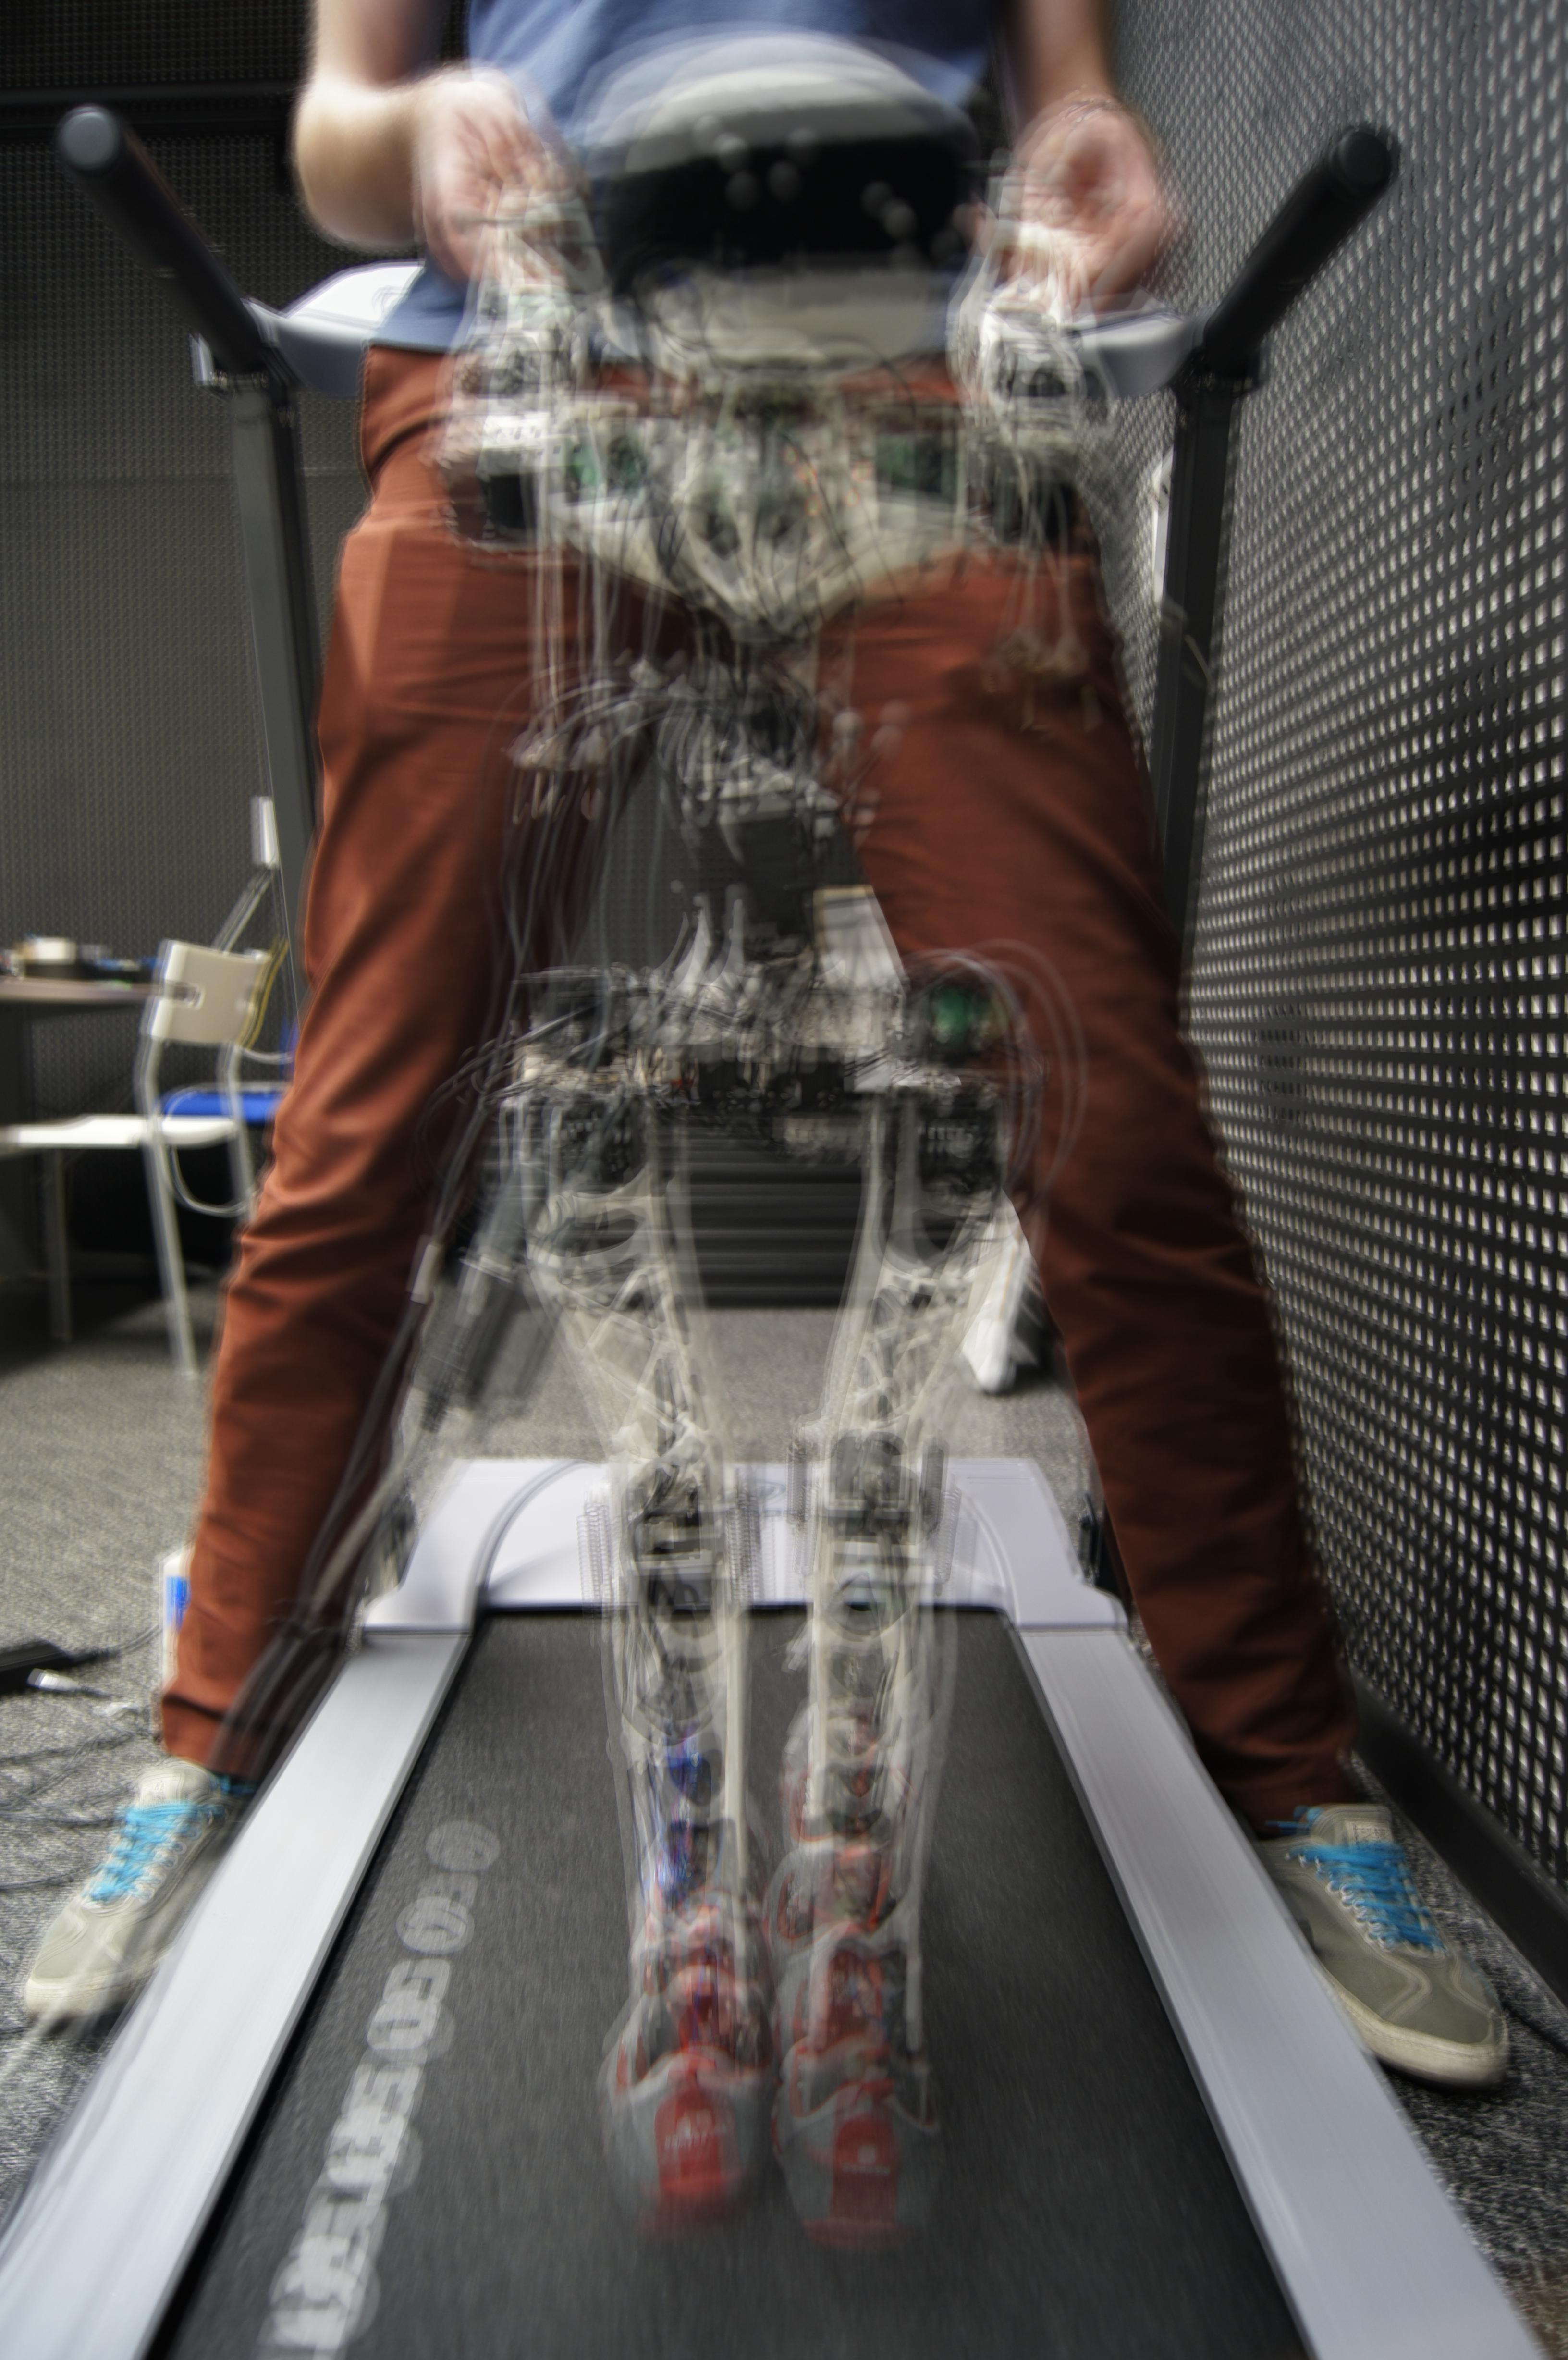
\includegraphics[width=0.45\linewidth]{marche_bended.jpg}}
    \hfil
    \subfloat[][straight thigh]{\label{fig:poppy_walking_straight}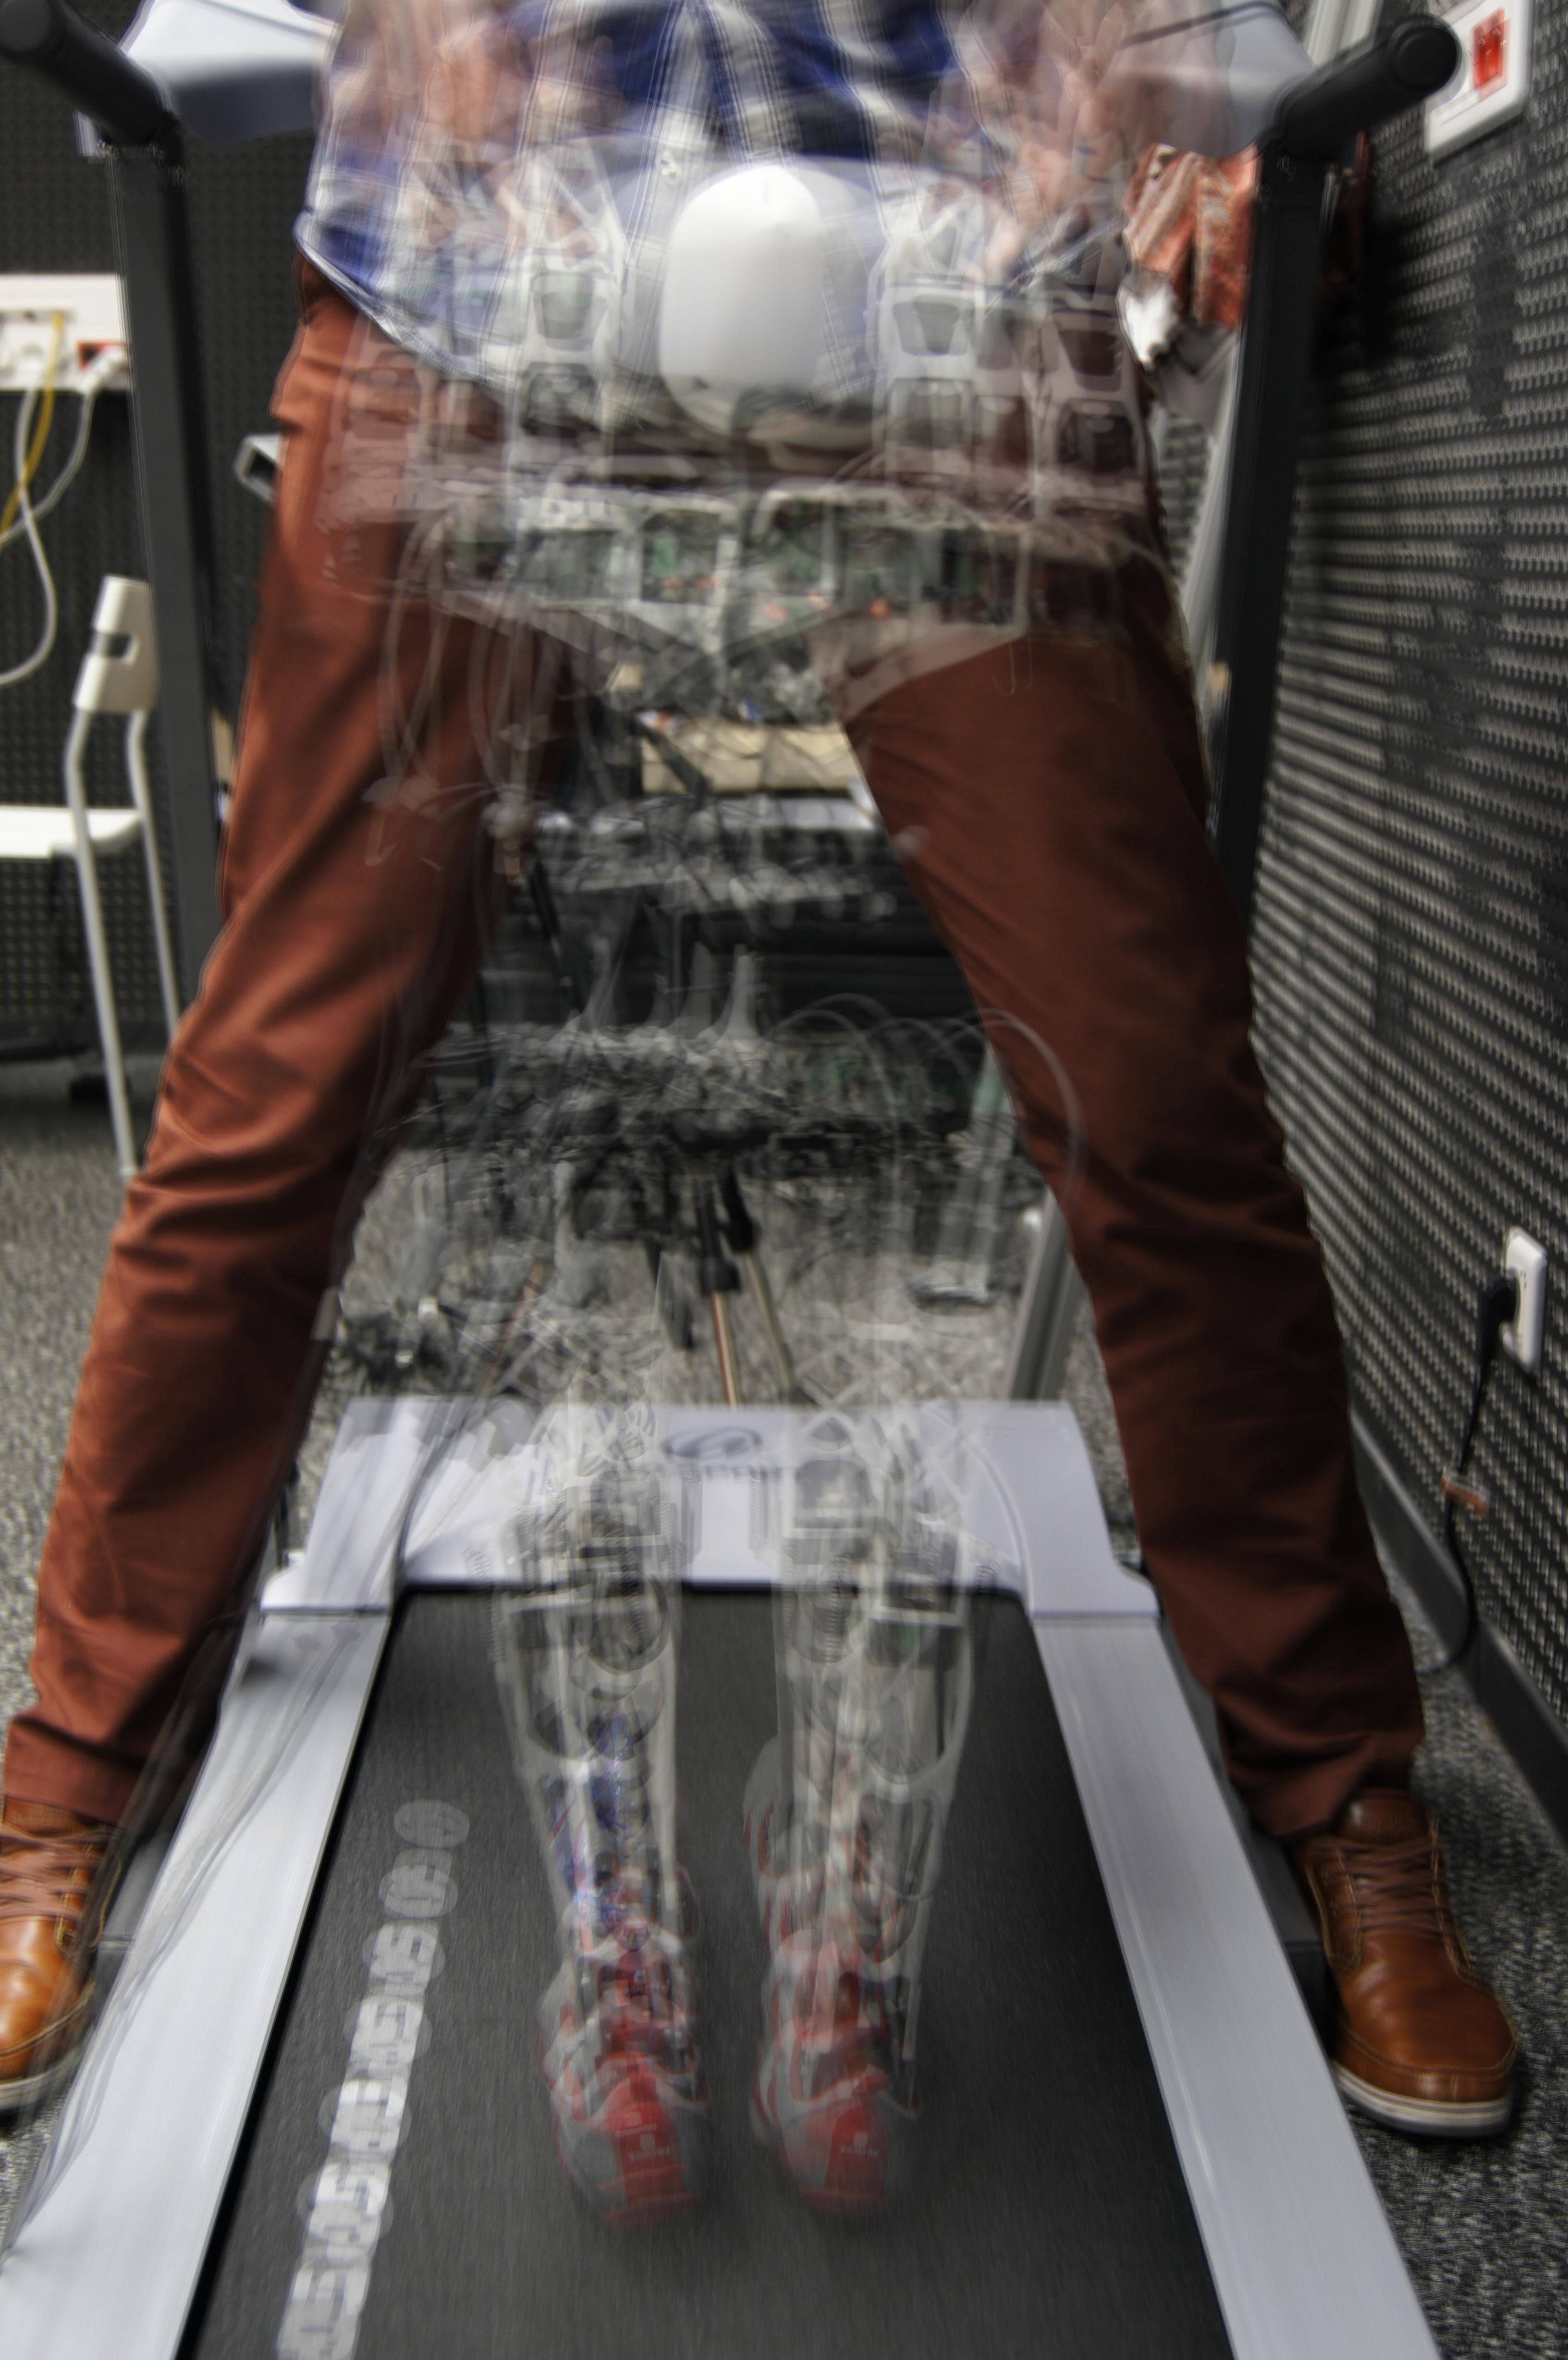
\includegraphics[width=0.45\linewidth]{marche_straight.jpg}}
    \caption{Five pictures have been taken while Poppy was walking and were stacked to obtain a qualitative view of the difference in the walking behavior in function of the morphology of the thigh.}
    \label{fig:poppy_walking_compared}
\end{figure}

% subsection experiments (end)
\subsection{results} % (fold)
\label{sub:results}
We have presented the morphological properties of a new humanoid robot platform named Poppy~\cite{lapeyre2013poppy}.
In this paper, we focus on the shape of the Poppy thigh and its effect on the robot dynamic.
We studied the role of the morphology in the reduction and simplification of the control needed to performs complex task such as biped walking.
We have presented the simple theoretical model we used for the design of Poppy thigh based on the inverse pendulum dynamic.
We have conducted experiments to evaluate the improvements of the bended thigh on the real robot dynamic and compare it with the model.
Thanks to the conception of Poppy allowing easy, cheap and fast morphology modifications, we were able to try another thigh design.
We also use a pair of straight thighs which is a more classical approach in humanoid conception.
The experimental comparison of the two thighs design confirmed the theoretical results, the bio-inspired thigh design improves Poppy dynamic on two main points useful for biped walking:
\begin{itemize}
    \item It reduces the falling velocity by almost 60\% when the robot is on one foot (single support phase).
    \item It reduces by 30\% the lateral motion needed to transfer the mass of the robot from one foot to the other (double support phase).
\end{itemize}
It is really interesting to note that such a small modification of the robot morphology has a very significant impact on the robot behavior.

These results are interesting but they do not reflect the actual Poppy dynamic while it is walking.
To evaluate the effect of the bended thigh on the biped locomotion, we conducted a third experiment where Poppy is walking on a treadmill.
In this experiment, we show that the bended thigh has an effect on a complex dynamic task such as the biped locomotion: it reduces the motion amplitude on the upper body of 45\% and increase the head stability of 30\%.
We choose these metrics due to our experimental constraints (fixed speed, social guidance) as a qualitative evaluation of the walking gait.
Moreover it provides us with an intuitive, yet incomplete evaluation of the walking.
Many other measures could have been chosen or combined such as speed, energy consumption or robustness to external perturbations.
It is still complicated to understand which metric is the most adapted for the robotic biped locomotion.
As human being is trained to recognize biped gait, users can provide guidance to the robot for both safety of exploration and evaluation of the walking behavior.

We will thus, in our future work, study the role of morphology in the learning of biped locomotion through this interaction.
Thanks to its multi-articulated and compliant spine (see Fig.~\ref{fig:poppy_features}), users physically induce motion in the trunk motors while they are guiding Poppy.
We could imagine learning this motion needed to generate the mass transfer during the walking gait.
Also, as the upper motions of Poppy with the bended thigh are small, we can imagine that the learning will be simplified.
An other interesting aspect concerns the evaluation of the right walking metrics to optimize.
As the guidance given by users is safe and provides good demonstrations of a "correct" walking gait, the robot can record a large amount of useful data to create a representation of the right walking behavior and find an adapted metric to evaluate its learning performances.

Last but not least, Poppy was conceived while considering issues of dissemination and was optimized to be very accessible (i.e.
cheap and easy to assemble).
Thus the whole Poppy drawing and software will be shortly released under OpenSource license for academics.
They will be able to reproduce the results obtained in this article, investigate other morphologies or use it as a test-bench for learning algorithms and human-robot interaction.
% subsection Results (end)


\section{Exploring foot and ankle shape for biped locomotion} % (fold)
\textbf{TODO}

% chapter exploring_the_role_of_morphology (end)
